%%「論文」,「レター」,「レター(C分冊)」,「技術研究報告」などのテンプレート
%% v3.3 [2020/06/02]

\documentclass[technicalreport]{ieicej}
\usepackage[dvipdfmx]{graphicx,xcolor}
\usepackage{float}
\usepackage[fleqn]{amsmath}
\usepackage{newtxtext}% 英数字フォントの設定を変更しないでください
\usepackage[varg]{newtxmath}% % 英数字フォントの設定を変更しないでください
\usepackage{latexsym}
\usepackage{listings}
\usepackage{xurl}
\usepackage{fancyvrb}
\usepackage{multirow}
\usepackage{array}
\usepackage[section]{placeins} % make sure all fig and table do not go to other sections
\usepackage{stfloats} % somehow avoid the possible blank page by fig or table
% \usepackage[normalem]{ulem}
% \useunder{\uline}{\ul}{}
%\usepackage{amssymb}


\renewcommand{\refname}{References} % To get english reference section heading
\renewcommand{\figurename}{Fig.} % To get english figure heading
\renewcommand{\tablename}{Table} % To get english table heading
\renewcommand\UrlFont{\rmfamily} % Fix url font

\lstset{%
    language={Python},
    basicstyle={\small},%
    identifierstyle={\small},%
    commentstyle={\small\itshape},%
    keywordstyle={\small\bfseries},%
    ndkeywordstyle={\small},%
    stringstyle={\small\ttfamily},
    frame={tb},
    breaklines=true,
    columns=[l]{fullflexible},%
    numbers=left,%
    xrightmargin=0zw,%
    xleftmargin=3zw,%
    numberstyle={\scriptsize},%
    stepnumber=1,
    showstringspaces=false,%
    numbersep=1zw,%
    lineskip=-0.5ex,%
    %moredelim=[is][\underbar]{_}{_},%
    keepspaces=true,%
    %escapechar=\@
}

% \jtitle{タイトル}
% \jsubtitle{}
\etitle{A Proposal of Speed-up Method for Fuzzy Search Process in Product Label Recognition System}
% \esubtitle{}
\authorlist{%
 \authorentry[chin-shiji@s.okayama-u.ac.jp]{陳 仕璽}{Shixi Chen}{okayama}
 \authorentry[funabiki@okayama-u.ac.jp]{舩曵 信生}{Nobuo Funabiki}{okayama}
 \authorentry[phvf8tn3@s.okayama-u.ac.jp]{坂上 正規}{Masaki Sakagami}{okayama}
 \authorentry[toshida.takashi@astrolab.co.jp]{土信田 高}{Takashi Toshida}{astrolab}
 \authorentry[suga@astrolab.co.jp]{菅 恒平}{Kohei Suga}{astrolab}
% \authorentry[メールアドレス]{和文著者名}{英文著者名}{所属ラベル}
}
\affiliate[okayama]{}
{Okayama University\hskip1em
Tsushimanaka 3-1-1, Okayama, 700--8530, Japan}
\affiliate[astrolab]{}
{Astrolab \hskip1em
Otemachi 2-6-2, Chiyoda, Tokyo, 100-0004, Japan}
%\affiliate[所属ラベル]{和文勤務先\\ 連絡先住所}{英文勤務先\\ 英文連絡先住所}
\jalcdoi{???????????}% ← このままにしておいてください

\begin{document}
% \begin{jabstract}
% %和文あらまし
% \end{jabstract}
% \begin{jkeyword}
% %和文キーワード
% \end{jkeyword}

\begin{eabstract}
    %background
    Recently, the {\em optical character recognition (OCR)} technology has been remarkably progressed to result in the high recognition rate due to the advancements of {\em deep learning techniques}. Besides, smartphones equipped with cameras have broadly spread among people around the world. As a result, the information acquisition from an object ravel using a smartphone camera can be a good choice as the easy and quick way.
    %problem to be solved
    However, the character recognition rate is still not $100\%$. Some characters are incorrectly recognized or missing in the recognition result. Then, if the correct characters to them have been stored as one record in a database, the {\em fuzzy search} can be applied to find the best matching record with the recognition result. Unfortunately, it will take long time if the database has a lot of records, because it spends much longer time to process one record. 
    %contribution
    In this study, we propose a speed-up method for the fuzzy search by limiting the processed records into possible ones where the part of the characters in the record is matching. 
    %evaluation
    For evaluations, we collect 396 photos of object ravels and their character recognition results, and apply our proposal to them. The results show that the proposal reduces the CPU time from $15.241sec$ to $0.984sec$ by limiting the number of search records into 0.24\% of all the records. However, the record hit rate is also reduced slightly from $91.16\%$ to $90.91\%$ whose improvement will be in future studies.
    
\end{eabstract}
\begin{ekeyword}
OCR, fuzzy search, regular expression, partial word matching
\end{ekeyword}
\maketitle

%+++++++++++++++++++++++++++++++++++++++++++++++
\section{Introduction}
    %background
    Recently, the {\em optical character recognition (OCR)} technology has been remarkably progressed to result in the high recognition rate due to the advancements of {\em deep learning techniques}. Besides, smartphones equipped with cameras have broadly spread among people around the world. As a result, the information acquisition from an object ravel using a smartphone camera can be a good choice as the easy and quick way.

    %problem to be solved
    However, the character recognition rate is still not $100\%$. Some characters are incorrectly recognized or missing in the recognition result. Then, if the correct characters to them have been stored as one record in a database, the {\em fuzzy search} can be applied to find the best matching record with the recognition result. Unfortunately, it will take unacceptably long time if the database has a lot of records, because it spends much longer time to process one record. 

    %contribution
    In this study, we propose a speed-up method for the fuzzy search by limiting the processed records into possible ones where the part of the characters in the record is matching. 
    We divide one alphanumeric string into two halves. For each half, we use partial matching to query in the database, to find out records containing either half of the divided string. By dividing into two halves, we can ensure the correct model is in the matched range even if there is one incorrectly recognized or missing character in the recognition result. Then we perform {\em fuzzy search} in this matched range only instead of the whole database. 

    %evaluation
    For evaluations, we collect 396 photos of object ravels and their character recognition results, and apply our proposal to them. The results show that the proposal reduces the CPU time from $15.241sec$ to $0.984sec$ by limiting the number of search records into 0.24\% of all the records. However, the record hit rate is also reduced from $91.16\%$ to $90.91\%$ whose improvement will be in future studies.
    Still, there are few cases which took longer than average time and not as fast as expected. With the longest searching time of over 13 seconds, our test result indicates that we can still do more to further improve this method.

    %contents
    The rest of this paper is organized as follows:

    Section \ref{sec:preliminary} shows preliminary technologies to this study.

    Section \ref{sec:proposal} presents the speed-up method.

    Section \ref{sec:evaluation} shows the evaluation results.

    Finally, Section \ref{sec:conclusion} concludes this paper with future works.


%+++++++++++++++++++++++++++++++++++++++++++++++
\section{Preliminary}
\label{sec:preliminary}
    In this section, we introduce preliminary technologies of our study in this paper.

    \subsection{Levenshtein Distance}
        Levenshtein is an algorithm to calculate {\em mininum edit distace (MED)} \cite{fuzzywuzzy-guidence}. The Levenshtein distance is a string metric for measuring the difference between two sequences. Informally, the Levenshtein distance between two words is the minimum number of single-character edits (insertions, deletions or substitutions) required to change one word into the other. \cite{levenshtein}

        The Levenshtein distance between two strings a and b is calculated by:

        \[
            \operatorname{lev}(a, b)=\left\{\begin{array}{ll}
            |a| & \text { if }|b|=0 \\
            |b| & \text { if }|a|=0 \\
            \operatorname{lev}(\operatorname{tail}(a), \operatorname{tail}(b)) & \text { if } a[0]=b[0] \\
            1+\min \left\{\begin{array}{l}
            \operatorname{lev}(\operatorname{tail}(a), b) \\
            \operatorname{lev}(a, \operatorname{tail}(b)) \\
            \operatorname{lev}(\operatorname{tail}(a), \operatorname{tail}(b))
            \end{array}\right. & \text { otherwise. }
            \end{array}\right.
        \]

    \subsection{FuzzyWuzzy}
        FuzzyWuzzy is a Python library useing Levenshtein Distance to calculate the differences between sequences. It relies on the Difflib module. \cite{fuzzywuzzy}-\cite{fuzzywuzzy-git}

        We use the Simple Ratio method of FuzzyWuzzy to calculate the similarity between two strings.The similarity is an integer ranging from 0 to 100. When two strings are exactly the same, the similarity is 100. For a 5-character string, if we compare it with another string which has one character different, as shown in the following code, the similarity is 80.
        
        \begin{lstlisting}
>>> from fuzzywuzzy import fuzz
>>> fuzz.ratio("A1532", "A15B2")
80      \end{lstlisting}


        Here we can understand calculating Levenshtein Distance between two words is more complicated and takes much longer time than simply comparing if the two words are identical.


%+++++++++++++++++++++++++++++++++++++++++++++++
\section{Proposal of Speed-up Method}
\label{sec:proposal}
    In this section, we propose the speed-up method for the Fuzzy search process in the product label recognition system.

    \subsection{System Overview}
        Our system is that user take a picture and give it to the system, the system will give the correct model of the product with the help of a prepared master DB.

        In the proposal, first, {\em optical character recognition (OCR)} is used to convert the picture into text. Second, we use a regular expression to filter and extract all alphanumeric strings which have possibility to be model text from the OCR result. Then, we divide the alphanumeric strings into two halves, and use partial word matching to pick model texts containing either half from the master database, which is pre-prepared and contains a large number of product models. Finally, we do fuzzy search in all the models picked, to find model texts most similar to any of the alphanumeric strings, which are the most possible model. 
        
    \subsection{System Input}
    \label{sec:algorithm.ocrregex}
        Our input are picture of product labels and a prepared master database.

        \subsubsection{Product Labels}
        \label{sec:label-request}

            The picture must be taken from the front of the product label and ensure that the ambient light is good so that the text on the label is clearly identifiable and try to avoid reflections. As the brightness, contrast, or other environmental condition when the pictures of product labels are taken changes, the accuracy of recognition can fluctuate significantly. The picture can be simply taken by smart phones or digital cameras. Like the picture shown in figure \ref{fig:label-exp}, we should take the label only with as few unrelated backgrounds as possible.

            \begin{figure}[t] 
                \begin{center}
                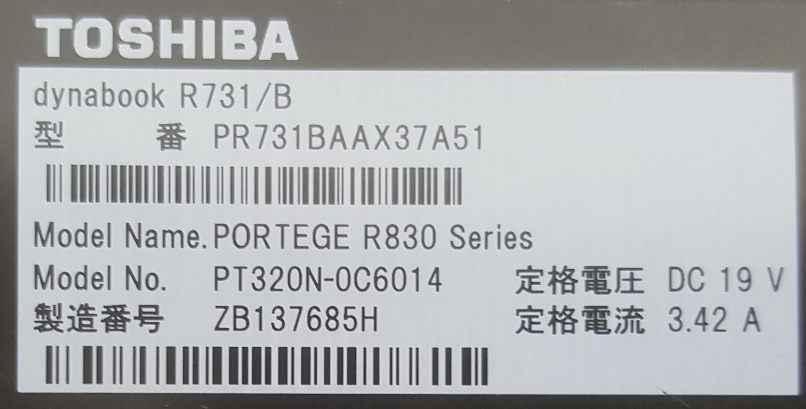
\includegraphics[width=0.48\textwidth]{figure/label-exp.png}
                \end{center}
                \caption{An example picture of product label accepted by our system}
                \label{fig:label-exp}
            \end{figure}


        \subsubsection{Master Database}
            We have a {\em master database} containing a lot of prepared model texts. As shown in figure \ref{fig:db-sample}, this database is prepared in advance and should cover as many product models as the system may see in practice. The database is used for correcting possible OCR mistake and make sure the result model really exists. 

            \begin{figure}[t] 
                \begin{center}
                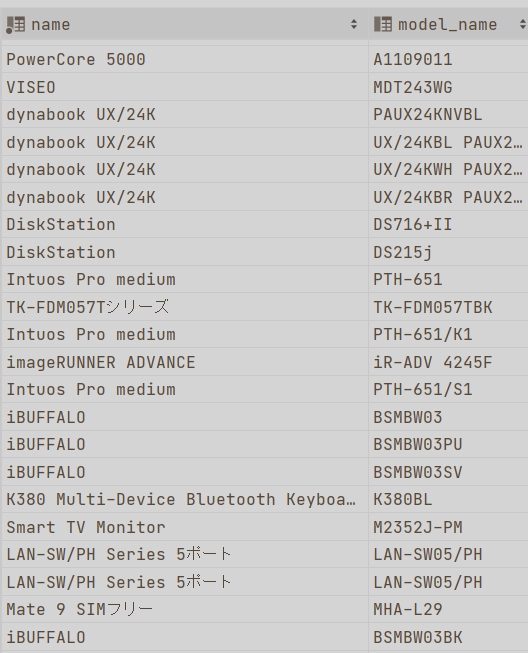
\includegraphics[width=0.48\textwidth]{figure/db-sample.png}
                \end{center}
                \caption{Part of the master database content}
                \label{fig:db-sample}
            \end{figure}

    
    \subsection{System Output}
        Our purpose is to output the model of the product in the picture. As shown in figure \ref{fig:result-sample}, the output is a list sorted by matching rate from high to low. The matching rate is an integer ranging from 0 to 100. When the OCR result text is identical as the model in a database record, the matching rate should be 100. The most possible model is the first one.

        \begin{figure}[t] 
            \begin{center}
        \begin{BVerbatim}
Matched Model:
{
    "EX-LD2071TB": 100,
    "EX-LDGC271TB": 87,
    "EX-LD2071TNV": 87,
    "EX-LDQ271DB": 82,
    "EX-LDH271DB": 82,
    "100-MR140": 71,
    "100-LA024": 71
}
        \end{BVerbatim}
        \end{center}
            \caption{Sample result list of the system}
            \label{fig:result-sample}
        \end{figure}


    \subsection{Conventional Method}
        In the conventional method, we use OCR, regular expression matching, and fuzzy search to get the result list.

        \subsubsection{OCR}
            First, OCR is used to convert the picture into text. OCR simply convert all the contents on the product label into text.
        

        \subsubsection{Regular Expression Matching}
            Second, we use a regular expression to filter and extract all alphanumeric strings which have possibility to be model text from the OCR recognition result. As most model text are alphanumeric strings, this step can filter out all other contents unrelated to model from the label.

            The regular expression we use:

            \begin{center}
            \begin{BVerbatim}
[ :]*((?=[a-zA-Z0-9\-\/\(\)]*[0-9])
[a-zA-Z0-9\-\/\(\)]{4,})[ ,.]*
            \end{BVerbatim}
            \end{center}
    
            The {\em [ :]*} in the beginning is set to exclude any possible guiding space or colon before the alphanumeric string we need.

            Then we have a long expression in brackets: {\em ((?=[a-zA-Z0-9$\backslash$-$\backslash$/$\backslash$($\backslash$)]*[0-9])[a-zA-Z0-9$\backslash$-$\backslash$/$\backslash$($\backslash$)]\{4,\}) }. Here the {\em (?=[a-zA-Z0-9$\backslash$-$\backslash$/$\backslash$($\backslash$)]*[0-9])} is called positive lookahead in regular expression, which asserts the following alphanumeric string, should be ending with a number. This positive lookahead just indicates what the following string should be like, but it does not actually pick any string, so the string we pick may contain a number in the middle rather than at the end. The following {\em [a-zA-Z0-9$\backslash$-$\backslash$/$\backslash$($\backslash$)]\{4,\})} is the one who actually picks a string more than 4 characters in length, containing letters, numbers, brackets, hyphen, or slashes, but not spaces.

            In other words, this part means, the alphanumeric string we want must be more than four characters in length, containing letters, numbers, brackets, hyphen, or slashes.

            Finally we have {\em [ ,.]*} in the end, which is used to exclude any possible following space, comma, or dot after the alphanumeric string we need, and make sure the string ends at the correct position.


        \subsubsection{Fuzzy Search in Master Database}
            Then, we do fuzzy search in all the records in the master database, to find model texts most similar to any of the alphanumeric strings, which are the most possible real model. This can tolerate OCR recognition errors. Specifically in this proposal, we use {\em FuzzyWuzzy} to calculate the similarity between two strings.
            
            With Fuzzy Search, for each identified alphanumeric string that may be model text, we compare it with all the model texts recorded in the master database, to calculate their similarity. The several matching results (5 by default) with highest similarity among all results are taken as candidates for output, which can ensure a higher accuracy.

    \subsection{Proposal of Speed-up Method}
        In this subsection, we describe the details of the proposal of speed-up method: fuzzy search limited by partial word matching.


        \subsubsection{Half Divided String}
            Before doing fuzzy search, we divide the matched alphanumeric strings into two halves from the center of the string.

        \subsubsection{Partial Word Matching}

            For the OCR errors of model text, in most cases, the number of incorrectly recognized characters may not exceed one.

            Thus we divide one alphanumeric string into two halves. For each half, partial matching is performed. Like in table \ref{table:half_matching}. We use partial matching rather than forward or backward matching so that we can avoid OCR text missing.

            In this way, if the misrecognized character is in the second half, the first half is a correct recognition. Partial matching can ensure that the completely matched correct model from the master database is included in the matching result. Conversely, if the misrecognized character is in the first half, partial matching can also help us to match the correct model.
            
            Let the original label text be “MX1234567” and the OCR result be “MX12345b7”, with one error. As shown in table \ref{table:half_matching}, it is divided into “MX123” and “45b7”. The matching result will contain the correct “MX1234567” model and together with some other models sharing the same half with less similarity, then output all of them into the result list.

            \begin{table}[tb]
                \caption{Half divided string and its matching results}
                \label{table:half_matching}
                \begin{center}
                    \begin{tabular}{c|c|c}
                    \Hline
                    origional label text & \multicolumn{2}{c}{MX1234567} \\ 
                    \hline
                    OCR result & \multicolumn{2}{c}{MX12345{\em b}7} \\ 
                    \hline
                    half divided strings & \_\_MX123\_\_ & \_\_45{\em b}7\_\_ \\
                    \hline
                    matching results & \begin{tabular}{c}MX123\underline{4567}\\MX123\underline{5678}\\\underline{P}MX123\underline{5678}\\...\end{tabular} & (no result)) \\
                    \Hline
                    \end{tabular}
                \end{center}
            \end{table}
        
%+++++++++++++++++++++++++++++++++++++++++++++++
\section{Evaluation}
\label{sec:evaluation}
    In this section, we evaluate the proposal. 

    \subsection{Photo Source}
        We took more than 400 photos to perform the test, and we used 396 of them which match the photo request described in section \ref{sec:label-request}.

    \subsection{Regular Expression Used for Matching}

        \begin{figure}[t] 
            \begin{center}
            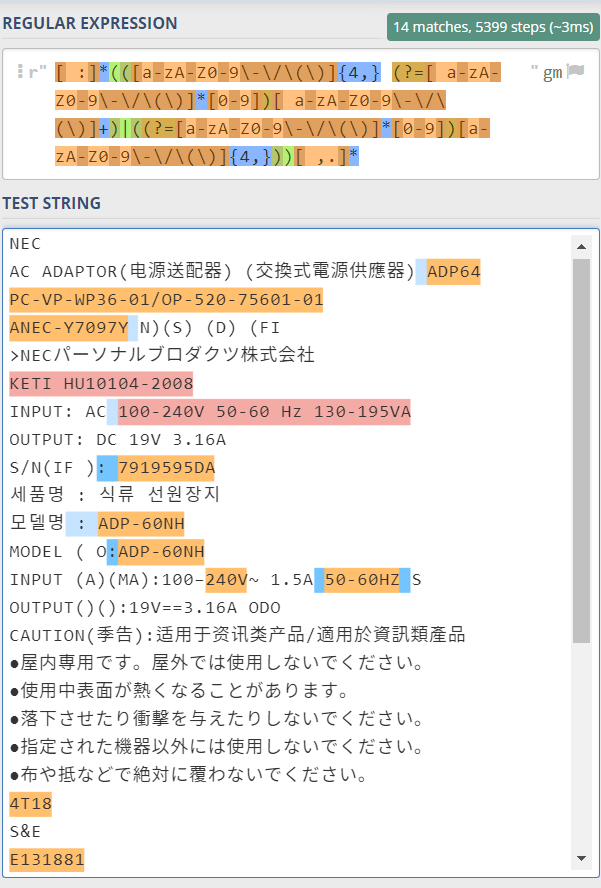
\includegraphics[width=0.48\textwidth]{figure/result-regex.png}
            \end{center}
            \caption{An example of regular expression matching result}
            \label{fig:result-regex}
        \end{figure}

        As shown in figure \ref{fig:result-regex}, which is a test result using regex101\cite{regex101}. The green marks in test string are the alphanumeric strings matched. We can see that the correct model {\em ADP-60NH} is among the result. Although the same string is matched multiple times, we can remove the duplicate ones later.

    \subsection{Result}
            
        We conducted 396 searches in a master database with 553,887 records.

        \subsubsection{Regular Expression Matching Rate}

            \begin{table}[t]
                \caption{Regular expression matching result [DATA NEEDS CORRECTION]}
                \label{table:regex_result}
                \begin{center}
                    \begin{tabular}{c|c}
                    \Hline
                    Items Tested & 396 \\ 
                    % \hline
                    Correct Model Extracted in Results & 311 \\ 
                    % \hline
                    Correct Model Missed in Results & 85 \\ 
                    % \hline
                    Correct Extracting Rate (\%) & 78.54 \\ 
                    % \hline
                    Average Amount of Strings Extracted for One Item & 8.654 \\ 
                    % \hline
                    Mininum Amount of Strings Extracted for One Item & 1 \\ 
                    % \hline
                    Maximum Amount of Strings Extracted for One Item & 38 \\ 
                    \Hline
                    \end{tabular}
                \end{center}
            \end{table}

            As shown in table \ref{table:regex_result}, among all the tests, in most cases the alphanumeric string containing correct model is successfully extracted by our regular expression. The correct extracting rate is about 78.54\%. There are still 85 cases in which our regular expression failed to match the correct model. But this does not cause an overall failure because we still have fuzzy search to correct minor matching errors.
            
            The average amount of strings extracted for one item is 8.654. All these results will be used as keywords in later fuzzy search. The minimum amount of strings extracted for one item is 1, while the maximum is 38.

        \subsubsection{Speed-up Method for Fuzzy Search Process}

            The time consumed is shown in the table \ref{table:methods_compare}.
    
            \begin{table*}[t]
                \caption{Performance result using different searching methods}
                \label{table:methods_compare}
                \begin{center}
                    \begin{tabular}{c|cc}
                    \Hline
                    search method &
                        \begin{tabular}{c} Conventional Method \end{tabular} &
                        \begin{tabular}{c} Speed-up Method \end{tabular} \\ 
                    \hline
                    Recognized as the 1st candidate in matching list &
                        340 & 339\\ 
                    \hline
                    Recognized in top 5 candidates in matching list &
                        361 & 360\\ 
                    \hline
                    Recognition Rate &
                        91.16\% & 90.91\%\\ 
                    \hline
                    Average Search Time &
                        15.241s & 0.984s \\ 
                    \hline
                    Median Search Time &
                        12.470s & 0.910s \\ 
                    \hline
                    Maximum Search Time &
                        64.273s & 3.004s \\ 
                    \hline
                    Average Search Range (DB Record Amount) &
                        553,887.00 & 1,347.68 \\
                    \Hline
                    \end{tabular}
                \end{center}
            \end{table*}

            Using conventional method, there are 340 cases in which the first candidate in result list is the correct one. In 361 cases the correct models are among the top 5 candidates. If we consider matched in the top 5 candidates as successful recognition, the recognition rate is 91.16\%. The average searching time for each item is 15.241s, median is 12.470s, while the maximum is 64.273s. As for each item we look up all the records in master DB, the average search range is the amount of records in DB, 553,887.
            
            Using speed-up method, there are 339 cases in which the first candidate in result list is the correct one. In 360 cases the correct models are among the top 5 candidates. If we consider matched in the top 5 candidates as successful recognition, the recognition rate is 90.91\%. The average searching time for each item is 0.984s, median is 0.910s, while the maximum is 3.004s. The average search range for each item, which means the amount of DB record we looked up in fuzzy search, is 1,347.68.

            \begin{table*}[t]
                \caption{Performance result using different searching methods}
                \label{table:slowest_rec}
                \begin{center}
                    \begin{tabular}{c|c|c|c|c|c|c|c}
                    \Hline
                        \begin{tabular}{c}Real \\Model\end{tabular} &
                        \begin{tabular}{c}Reuglar\\Expression\\Matching Results\end{tabular} &
                        \begin{tabular}{c}Reuglar\\Expression\\Matching Correct\end{tabular} &
                        \begin{tabular}{c}Partial Word\\Matching\\Costed Time (s)\end{tabular} &
                        \begin{tabular}{c}Fuzzy Search\\Total Costed\\Time (s)\end{tabular} &
                        \begin{tabular}{c}Fuzzy Search\\Range (DB\\Record Amount)\end{tabular} &
                        \begin{tabular}{c}Fuzzy\\Search\\1st matched\end{tabular} &
                        \begin{tabular}{c}Fuzzy Search\\top 5\\matched\end{tabular} \\ 
                    \Hline
                    DC35 & 14 & False & 0.26997 & 1.80353 & 24675 & False & False \\ 
                    \hline
                    DM-E25AW & 29 & True & 0.35329 & 2.41260 & 2912 & True & True \\ 
                    \hline
                    TPC-F026-SF & 23 & False & 0.33008 & 2.51139 & 6761 & True & True \\ 
                    \hline
                    K04A-WH & 38 & True & 0.46103 & 2.53164 & 5009 & True & True \\ 
                    \hline
                    MRO-GS8 & 22 & True & 0.31031 & 2.91033 & 3822 & True & True \\ 
                    \hline
                    NE-BS805-K & 33 & True & 0.40080 & 3.00420 & 5574 & True & True \\ 
                    \Hline
                    \end{tabular}
                \end{center}
            \end{table*}

            Among the Fuzzy Search limited by partial word matching results, the several experiments in which the time-consuming is significantly higher than the average time-consuming are as in the table \ref{table:slowest_rec}. We can see the time costed is up to 3.004s, with searching ranges of up to 24675 records.
    
            
%+++++++++++++++++++++++++++++++++++++++++++++++
\section{Conclusion}
\label{sec:conclusion}
    Using the speed-up method can effectively reduce the time into the acceptable range while increasing the accuracy rate to be close to that of the conventional method. With this method, we can take a balance between searching speed and mistake prevention for OCR text, and successfully limit the search range into over one thousand (about 0.24\% of all data amount). In most cases the search result would come out in only less than 2 seconds which is acceptable for users to wait.
    
    As shown in figure \ref{fig:graph-time} and \ref{fig:graph-recognized}, our speed-up method for fuzzy search is proved to be effective.

    \begin{figure}[t] 
        \begin{center}
        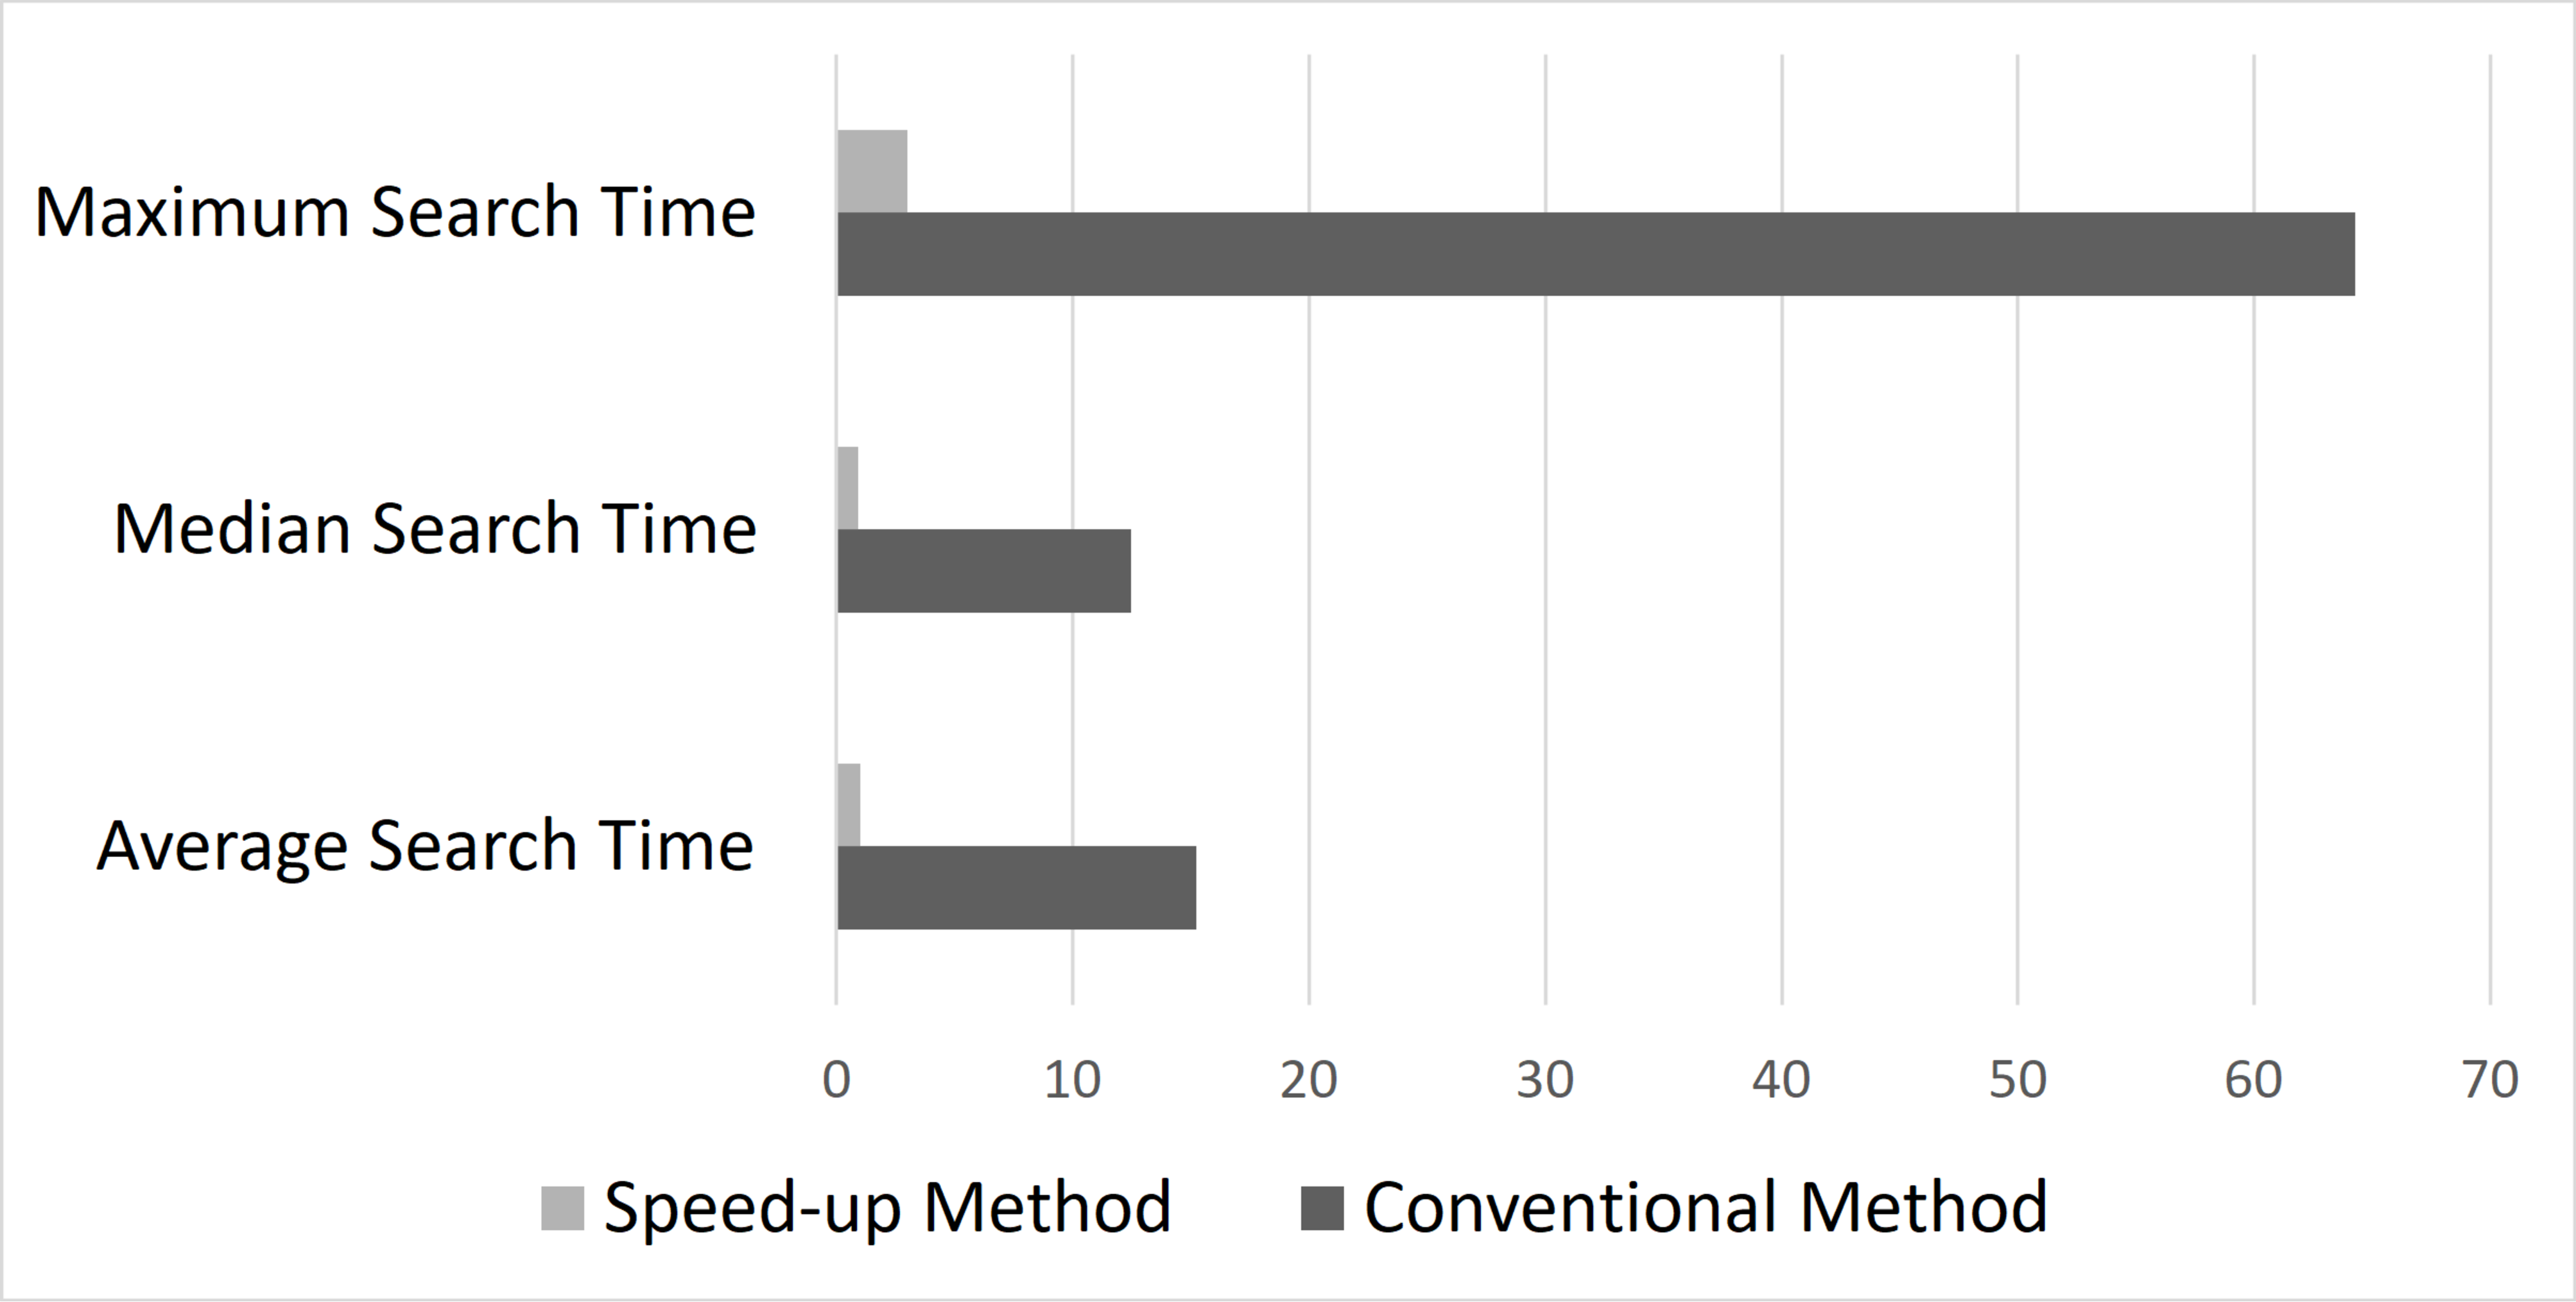
\includegraphics[width=0.48\textwidth]{figure/graph-time.pdf}
        \end{center}
        \caption{Search Time Comparation}
        \label{fig:graph-time}
    \end{figure}

    \begin{figure}[t] 
        \begin{center}
        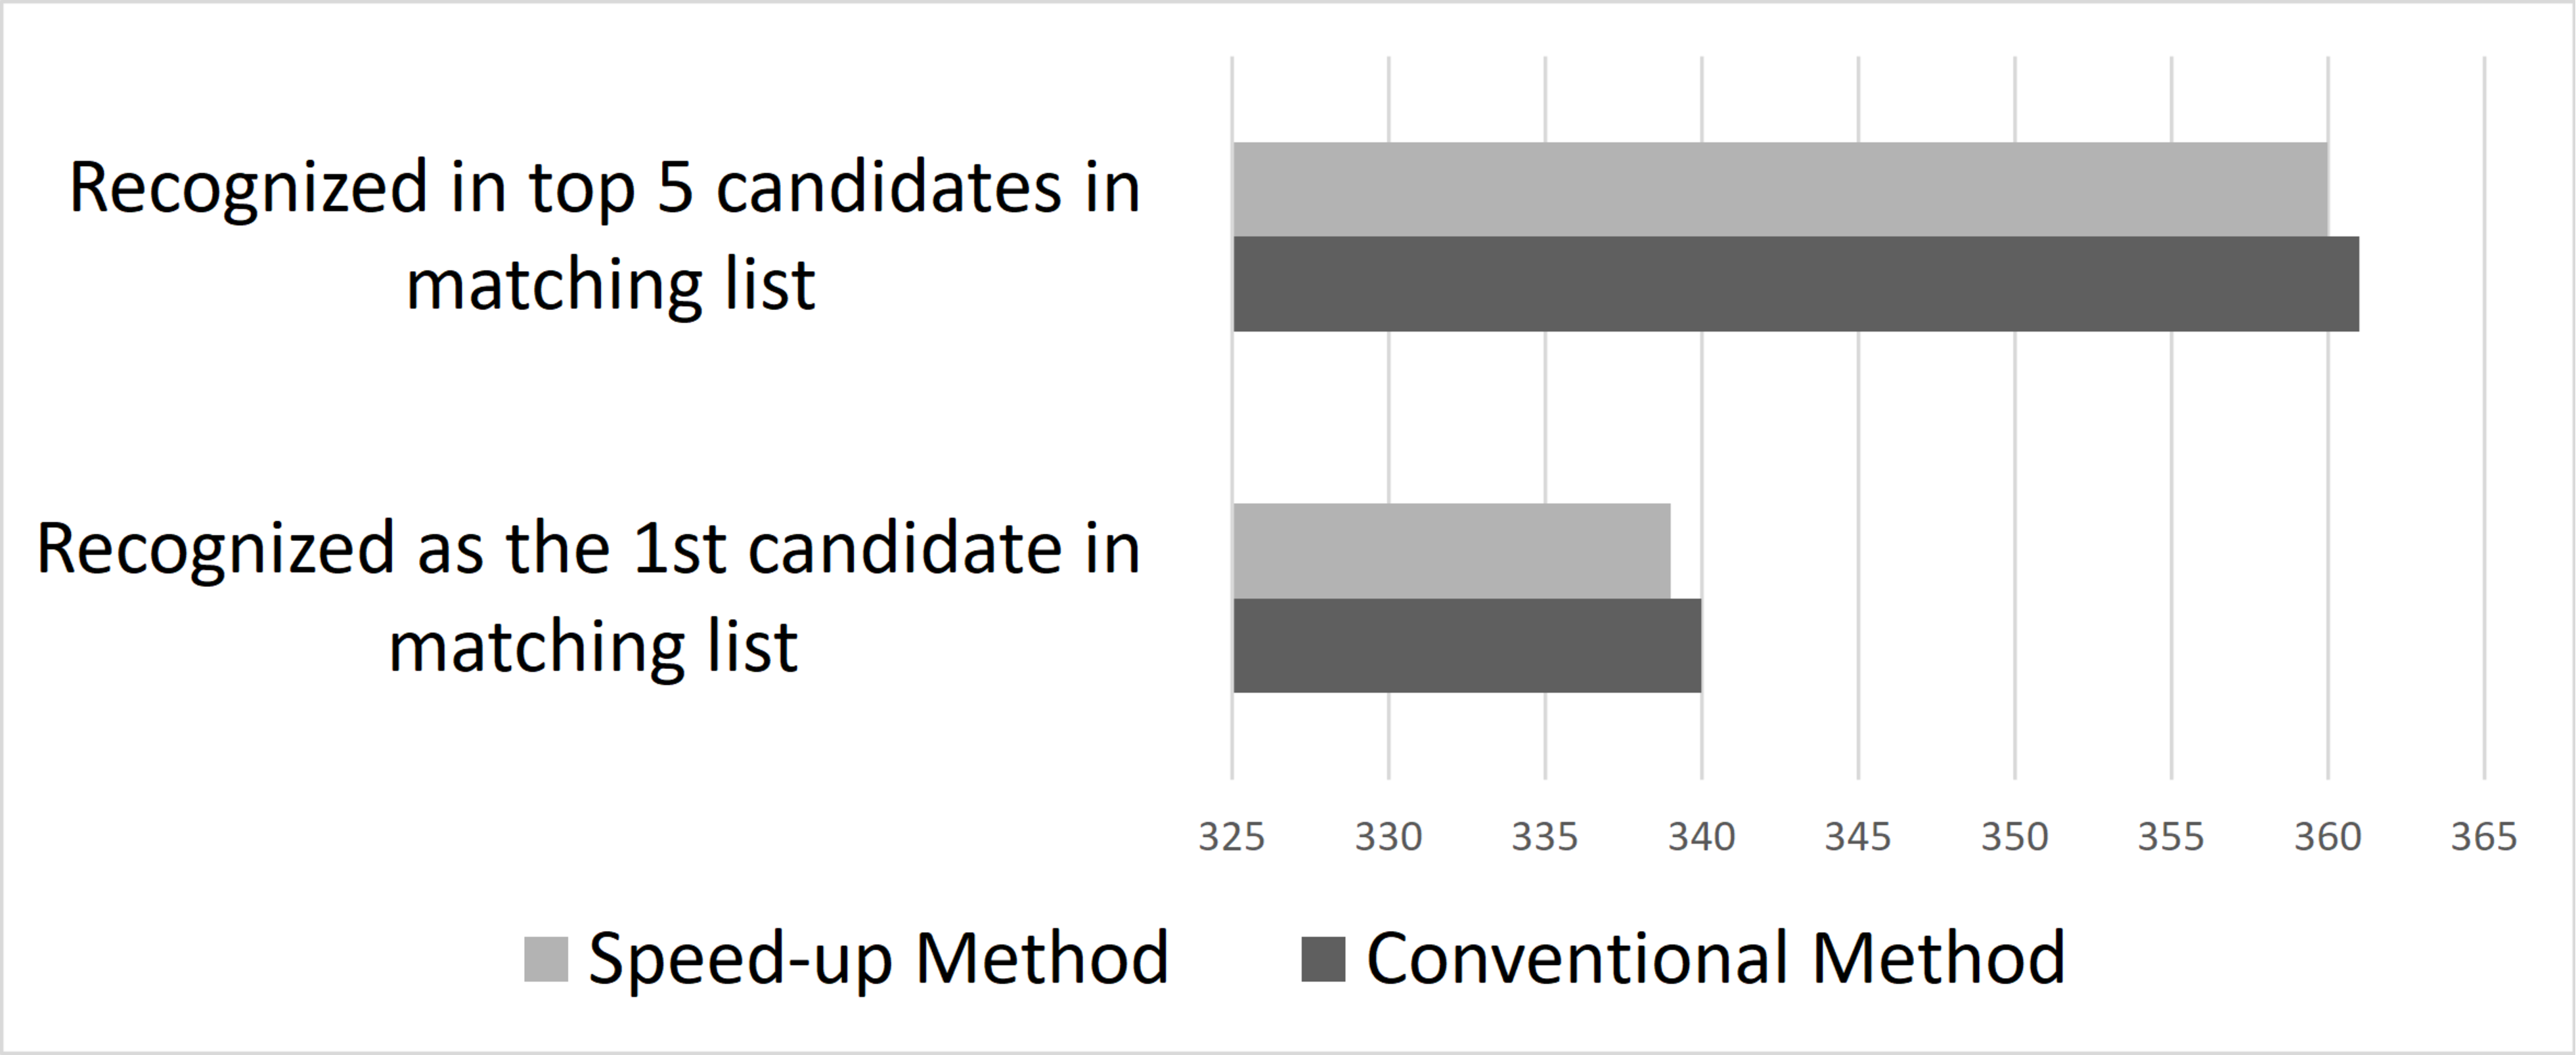
\includegraphics[width=0.48\textwidth]{figure/graph-recognized.pdf}
        \end{center}
        \caption{Search Time Comparation}
        \label{fig:graph-recognized}
    \end{figure}
    
    It can be seen from table \ref{table:slowest_rec} that for few cases, after the limitation of character recognition, the search range is still large, thus it took longer than average time and not as fast as expected. The longest searching time of over 3 seconds. This indicates that we can still do more to further improve this method.
    
    We consider that, for each record in the master database, we can add not only the model text information of the product, but also its brand or manufacturer information. Before doing fuzzy search, we can also use other recognition methods to match and analyze the text contained in the OCR results to determine the brand of the product, and use brand information matching to further limit the search range of fuzzy search for model texts, which may further improve searching performance.

    Also, for the result of regular expression shown in figure \ref{fig:result-regex}, we can see some alphanumeric strings unrelated with model also got matched. In future studies we need to find better patterns for regular expression to reduce unnecessary fuzzy searching.

    As our output is a list of most possible models in the product label, it is possible that there are several similar models with the same matching rate. How to correctly pick out the correct one is still to be studied.
    

%+++++++++++++++++++++++++++++++++++++++++++++++
%\bibliographystyle{sieicej}
%\bibliography{myrefs}
\begin{thebibliography}{99}% 文献数が10未満の時 {9}
    \bibitem{fuzzywuzzy-guidence}
    \url{https://towardsdatascience.com/fuzzywuzzy-fuzzy-string-matching-in-python-beginners-guide-9adc0edf4b35}
    
    \bibitem{levenshtein}
    \url{https://en.wikipedia.org/wiki/Levenshtein_distance}



    \bibitem{fuzzywuzzy}
    \url{https://chairnerd.seatgeek.com/fuzzywuzzy-fuzzy-string-matching-in-python/}

    \bibitem{fuzzywuzzy-git}
    \url{https://github.com/seatgeek/fuzzywuzzy}


    \bibitem{regex101}
    \url{https://regex101.com/}


    % \bibitem{Funabiki13} 
    % N. Funabiki, Y. Matsushima, T. Nakanishi, and N. Amano, "A Java programming learning assistant system using test-driven development method," \emph{IAENG Int. J. Comput. Sci.}, vol. 40, no.1, pp. 38-46, Feb. 2013.
    
    % \bibitem{Zaw15}
    % K. K. Zaw, N. Funabiki, and W.-C. Kao, "A proposal of value trace problem for algorithm code reading in Java programming learning assistant system," \emph{Inf. Eng. Express}, vol. 1, no. 3, pp. 9-18, Sep. 2015.
    
    % \bibitem{Funabiki17} 
    % N. Funabiki, Tana, K. K. Zaw, N. Ishihara, and W.-C. Kao, "A graph-based blank element selection algorithm for fill-in-blank problems in Java programming learning assistant system, \emph{IAENG Int. J. Comput. Sci.}, vol. 44, no. 2, pp. 247-260, May 2017.
    
    % \bibitem{cup}
    % CUP, \url{http://czt.sourceforge.net/dev/java-cup/manual.html}
    
    % \bibitem{scope}
    % Scope, https://www.codesdope.com/blog/article/scope-of-variables-in-c/
    
    % \bibitem{example}
    % \url{http://www.codebind.com/c-examples/}
    
    % \bibitem{triangle}
    % \url{https://brilliant.org/wiki/pascals-triangle/}
    
    % \bibitem{related1}
    % A. Kashihara, A. Terai, and J. Toyota, "Making fill-in-blank program problems for learning algorithm, " \emph{in Proc. Int. Conf. Comput. Edu.}, pp. 776-783, 1999.
    
    % \bibitem{related2}
    % J. Shinkai, Y. Hayase, and I. Miyaji, "A study of generation and utilization of fill-in-the-blank questions for programming education on Moodle, " \emph{IEICE Technical Report}, vol. 110, no. 263, pp. 7-10, 2010.
    
    % \bibitem{related3}
    % K. Terada, Y. Watanobe, "Automatic generation of fill-in-the-blank programming problems, " \emph{in Proc. IEEE Int. Symp. Embed. Mult./Many-core Sys.-on-Chip (MCSoC)}, pp. 187-193, 2019.
\end{thebibliography}

\end{document}

